%Set document format
\documentclass[11pt]{article}
\usepackage[margin=1in]{geometry}

%Set up packages
\usepackage{amsmath,amssymb,amsthm}
\usepackage{graphicx}
\usepackage{textcomp, gensymb}
\usepackage{float}
\usepackage{pdfpages}
\usepackage[hidelinks]{hyperref}
\usepackage{listings}
\usepackage{cancel}
\usepackage{subcaption}
\usepackage{caption}

\usepackage{mdframed}

\newcommand{\bm}{\boldsymbol}
\newcommand{\bI}{\mathbb{I}}
\newcommand{\bR}{\mathbb{R}}

\setlength\parindent{0pt}

\title{\bf Supersonic Flow Over a Diamond Airfoil}
\author{Group 2 : Andrew Doty, Buck Newberry, Andres Suniaga, David Valenzano \\[2mm] \textit{Dept. of Aerospace Engineering and Engineering Mechanics, The University of Texas at Austin}}
\date{November 19, 2024}

\begin{document}
\maketitle


\noindent\makebox[\textwidth]{\rule{\textwidth}{0.2pt}}
\tableofcontents
\noindent\makebox[\textwidth]{\rule{\textwidth}{0.2pt}}
\pagebreak

\section{Abstract}


\pagebreak

\section{Introduction}


\pagebreak

\section{Theory}
The basis for this report is the Schlieren imaging technique that takes advantage of the normally imperceptible changes in the index of refraction of gases that occur due to changes in destiny. Light from a point source is reflected and made parallel by a concave parabolic mirror. This light passes through a section of air and refracted light is disturbed from its straight path. Half of this disturbed light is blocked by a razors edge before it reaches a camera. The resulting image has the disturbed light showing up as brighter spots where it converges and darker spots where it has been diverged away from. This results in the image displaying the changes in the air's density like in the shocks and expansion fans in this report. 
\vspace{2.5mm}

Similarly important are the relations of shocks. If a compressible gas moves around an object, for low subsonic Mach numbers, it will simply flow around it. However, if that flow is going faster than the speed of sound and the change in properties like area are rapid, then a shock is formed. These changes in flow properties are non-isentropic as the changes in temperature and velocity are large within the shock itself. The specific relation used in this report are the oblique shock relations shown below:

\begin{equation*}
    \tan{(\theta)} = 2\cot{(\beta)}\dfrac{M_{1}^{2} \sin^{2}{(\beta)} - 1}{M_{1}^{2}(\gamma + \cos{(2\beta)}) + 2}
\end{equation*}
\vspace{2.5mm}

The $\theta$-$\beta$-$\text{Mach}$ relation for predicting the wave angle $\beta$ the shock will form at a given incoming Mach number $M_{1}$ and turn angle the flow is making $\theta$.

\begin{equation*}
    M_{1_{\text{N}}} = M_{1} \sin{(\beta)}
\end{equation*}

\begin{equation*}
    M_{2_{\text{N}}}^{2} = \dfrac{1 + \left(\dfrac{\gamma-1}{2}\right) M_{1_{\text{N}}}^{2}}{\gamma M^{2}_{1_{\text{N}}} - \left(\dfrac{\gamma-1}{2}\right)}
\end{equation*}

\begin{equation*}
    M_{2} = \dfrac{M_{2_{\text{N}}}}{\sin{(\beta - \theta)}}
\end{equation*}

The normal shock relation is used with the assumption that the change in Mach number across the shock only occurs to the normal portion of the flow. This is used to predict the post-shock Mach number $M_{2}$ given an incoming Mach number $M_{1}$ across an oblique shock. The change in static pressure across the shock is modeled by:

\begin{equation*}
    P_{2} = P_{1}\left[1 + \left(\dfrac{2\gamma}{\gamma + 1}\right) (M^{2}_{1_{\text{N}}} - 1)\right]
\end{equation*}

Where $P_{1}$ is the freestream static pressure before the shock and $P_{2}$ being the post shock static pressure.
\vspace{5mm}

Following the shock on the diamond airfoils will be a Prandtl-Meyer expansion fan for the flow going over the middle section of the diamond. The flow has to turn into and expand around an angle $\theta$ and the relation of the pre and post-fan Mach number is given by:

\begin{equation*}
    \theta = \nu(M_{2}) - \nu(M_{1})
\end{equation*}

\begin{equation*}
    \nu = \sqrt{\dfrac{\gamma + 1}{\gamma - 1}}\tan^{-1}{\left( \sqrt{\dfrac{\gamma-1}{\gamma+1}} (M^{2} - 1)   \right)} - \tan^{-1}{(\sqrt{M^{2} - 1})}
\end{equation*}

Where $\nu$ is a function of the flow's Mach number. The resulting Mach number can then give us the post-turn static pressure through the isentropic relations that connect a flow's Mach number to its properties since Prandtl-Meyer fans are isentropic and thus the stagnation properties are constant through the fan.

\begin{equation*}
    P_{0_{1}} = P_{1}\left[1 + (\dfrac{\gamma -1}{2}) M_{1}^{2} \right] ^{\frac{\gamma}{\gamma - 1}} = P_{0_{2}}
\end{equation*}

\begin{equation*}
    P_{2} = \dfrac{P_{0_{2}}}{\left[1 + (\dfrac{\gamma -1}{2}) M_{2}^{2} \right] ^{\frac{\gamma}{\gamma - 1}}}
\end{equation*}

The coefficients of sectional lift and drag are found from distributions of pressure across the 4 faces of the diamond to ascertain some lift and drag forces and then combined with the standard expressions of lift and drag:

\begin{equation*}
    l = \frac{1}{2}\rho_{\infty}U_{\infty}^{2}C_{l}c
\end{equation*}

\begin{equation*}
    d = \frac{1}{2}\rho_{\infty}U_{\infty}^{2}C_{d}c
\end{equation*}

Which then turn into:

\begin{equation*}
    C_{l} = \dfrac{1}{\gamma P_{\infty} M_{\infty}^{2} \cos{(\theta)}} \left[(P_{3} - P_{2})\cos{(\theta + \alpha)} + (P_{4}-P_{1})\cos{(\theta-\alpha)}\right]
\end{equation*}

\begin{equation*}
    C_{d} = \dfrac{1}{\gamma P_{\infty} M_{\infty}^{2} \cos{(\theta)}} \left[(P_{1} - P_{4})\sin{(\theta - \alpha)} + (P_{3} - P_{2})\sin{(\theta + \alpha)}\right]
\end{equation*}

Derivations of which can be found in the appendix of this report.$^{\hyperlink{derivations}{\text{A}}}$
\vspace{5mm}

The center of pressure for the airfoil are determined by:
\begin{equation*}
    \dfrac{CP_{x}}{c} = \dfrac{\frac{1}{4}(P_{1}-P_{3}) + \frac{3}{4}(P_{2} - P_{4})}{P_{1} - P_{3} + P_{2} - P_{4}}
\end{equation*}

\begin{center}
    if $\alpha = 0\degree \implies$ \(\left|\dfrac{CP_{x}}{c}\right|_{\alpha = 0\degree} = \dfrac{\frac{1}{4}P_{1} + \frac{3}{4}P_{2}}{P_{1} + P_{2}}\)
\end{center}

\begin{equation*}
    \dfrac{CP_{y}}{t} = \dfrac{P_{1} - P_{2} - P_{3} + P_{4}}{2(P_{1} - P_{2} + P_{3} - P_{4}}
\end{equation*}
\vspace{2.5mm}

Where the static pressures of the faces are:

\begin{figure}[H]
    \centering
    \includegraphics[width = 0.75\linewidth]{ReportImages/DiamondAirfoilSurfacePressures.png}
\end{figure}
\pagebreak

\section{Experimental Setup}

\pagebreak

\section{Results \& Discussion}

\subsection{Flow Images}
\begin{figure}[H]
    \centering
    \begin{subfigure}{0.475\linewidth}
        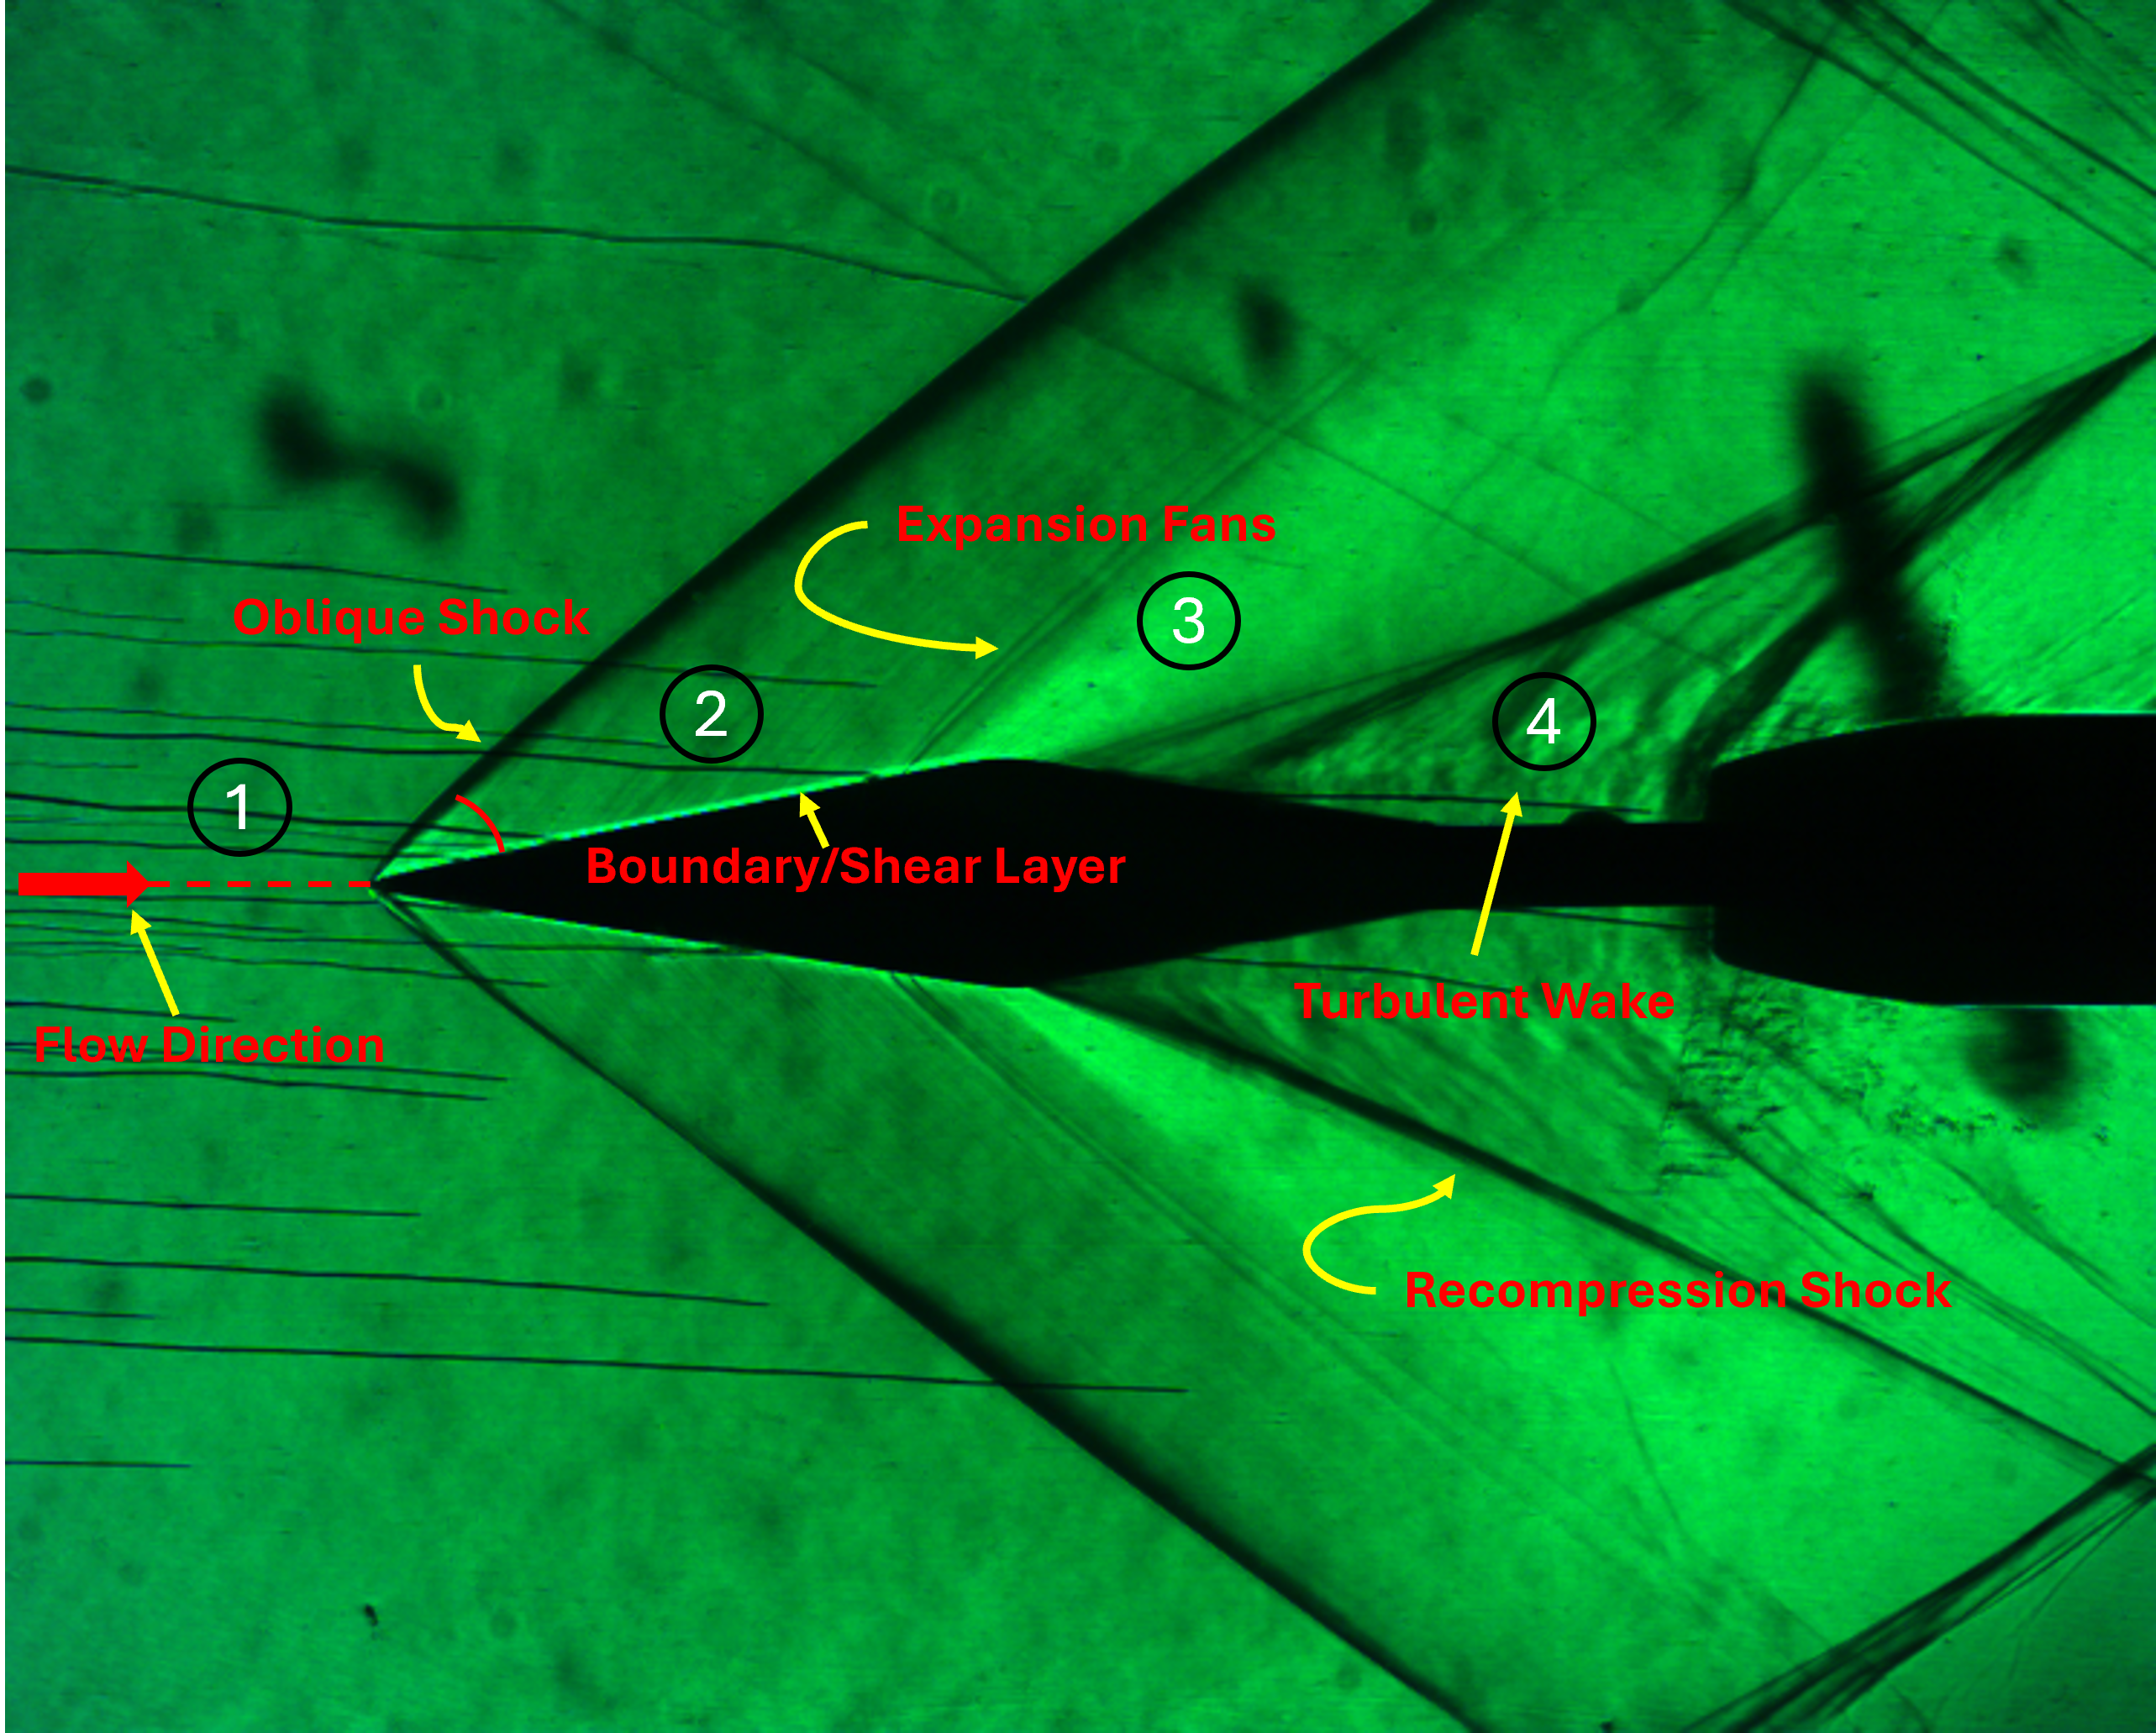
\includegraphics[width = \linewidth]{LabeledImages/Mach2_AoA0.png}
        \caption{Mach 2 flow at $0\degree$ angle of attack}
    \end{subfigure}
    \hspace{2.5mm}
    \begin{subfigure}{0.475\linewidth}
        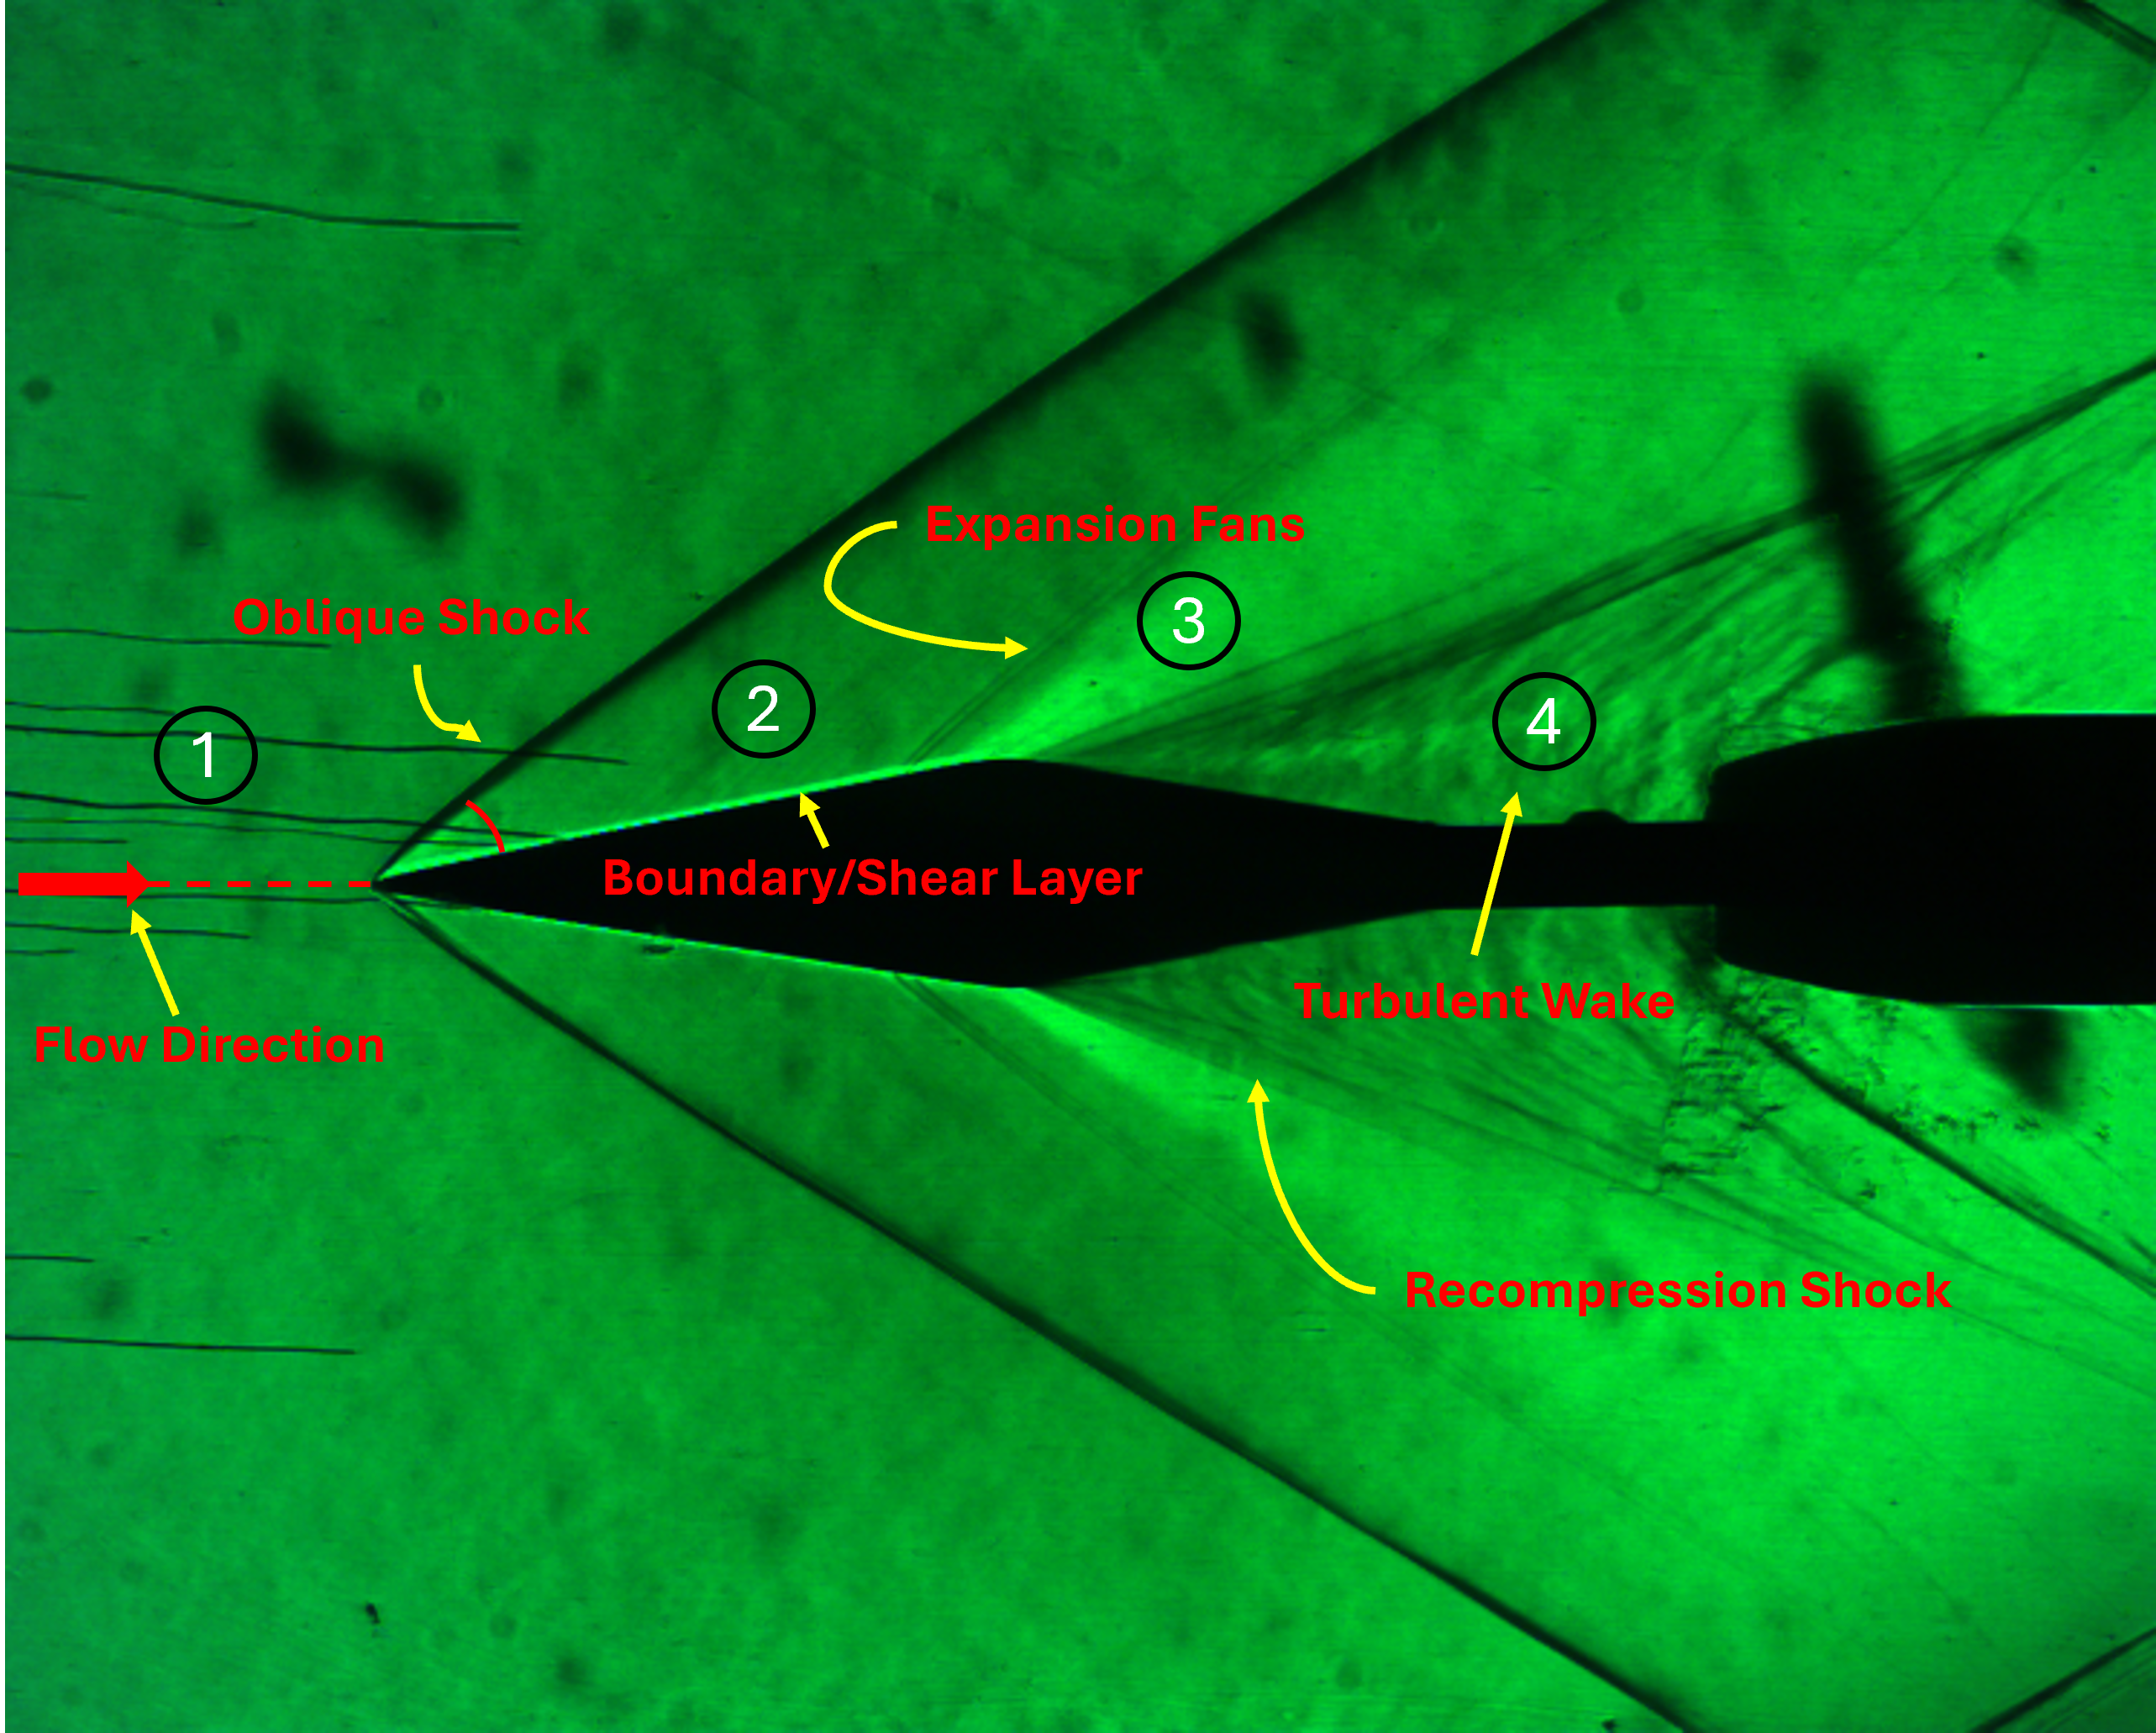
\includegraphics[width = \linewidth]{LabeledImages/Mach25_AoA0.png}
        \caption{Mach 2.5 flow at $0\degree$ angle of attack}
    \end{subfigure}
    \par\bigskip
    \begin{subfigure}{0.60\linewidth}
        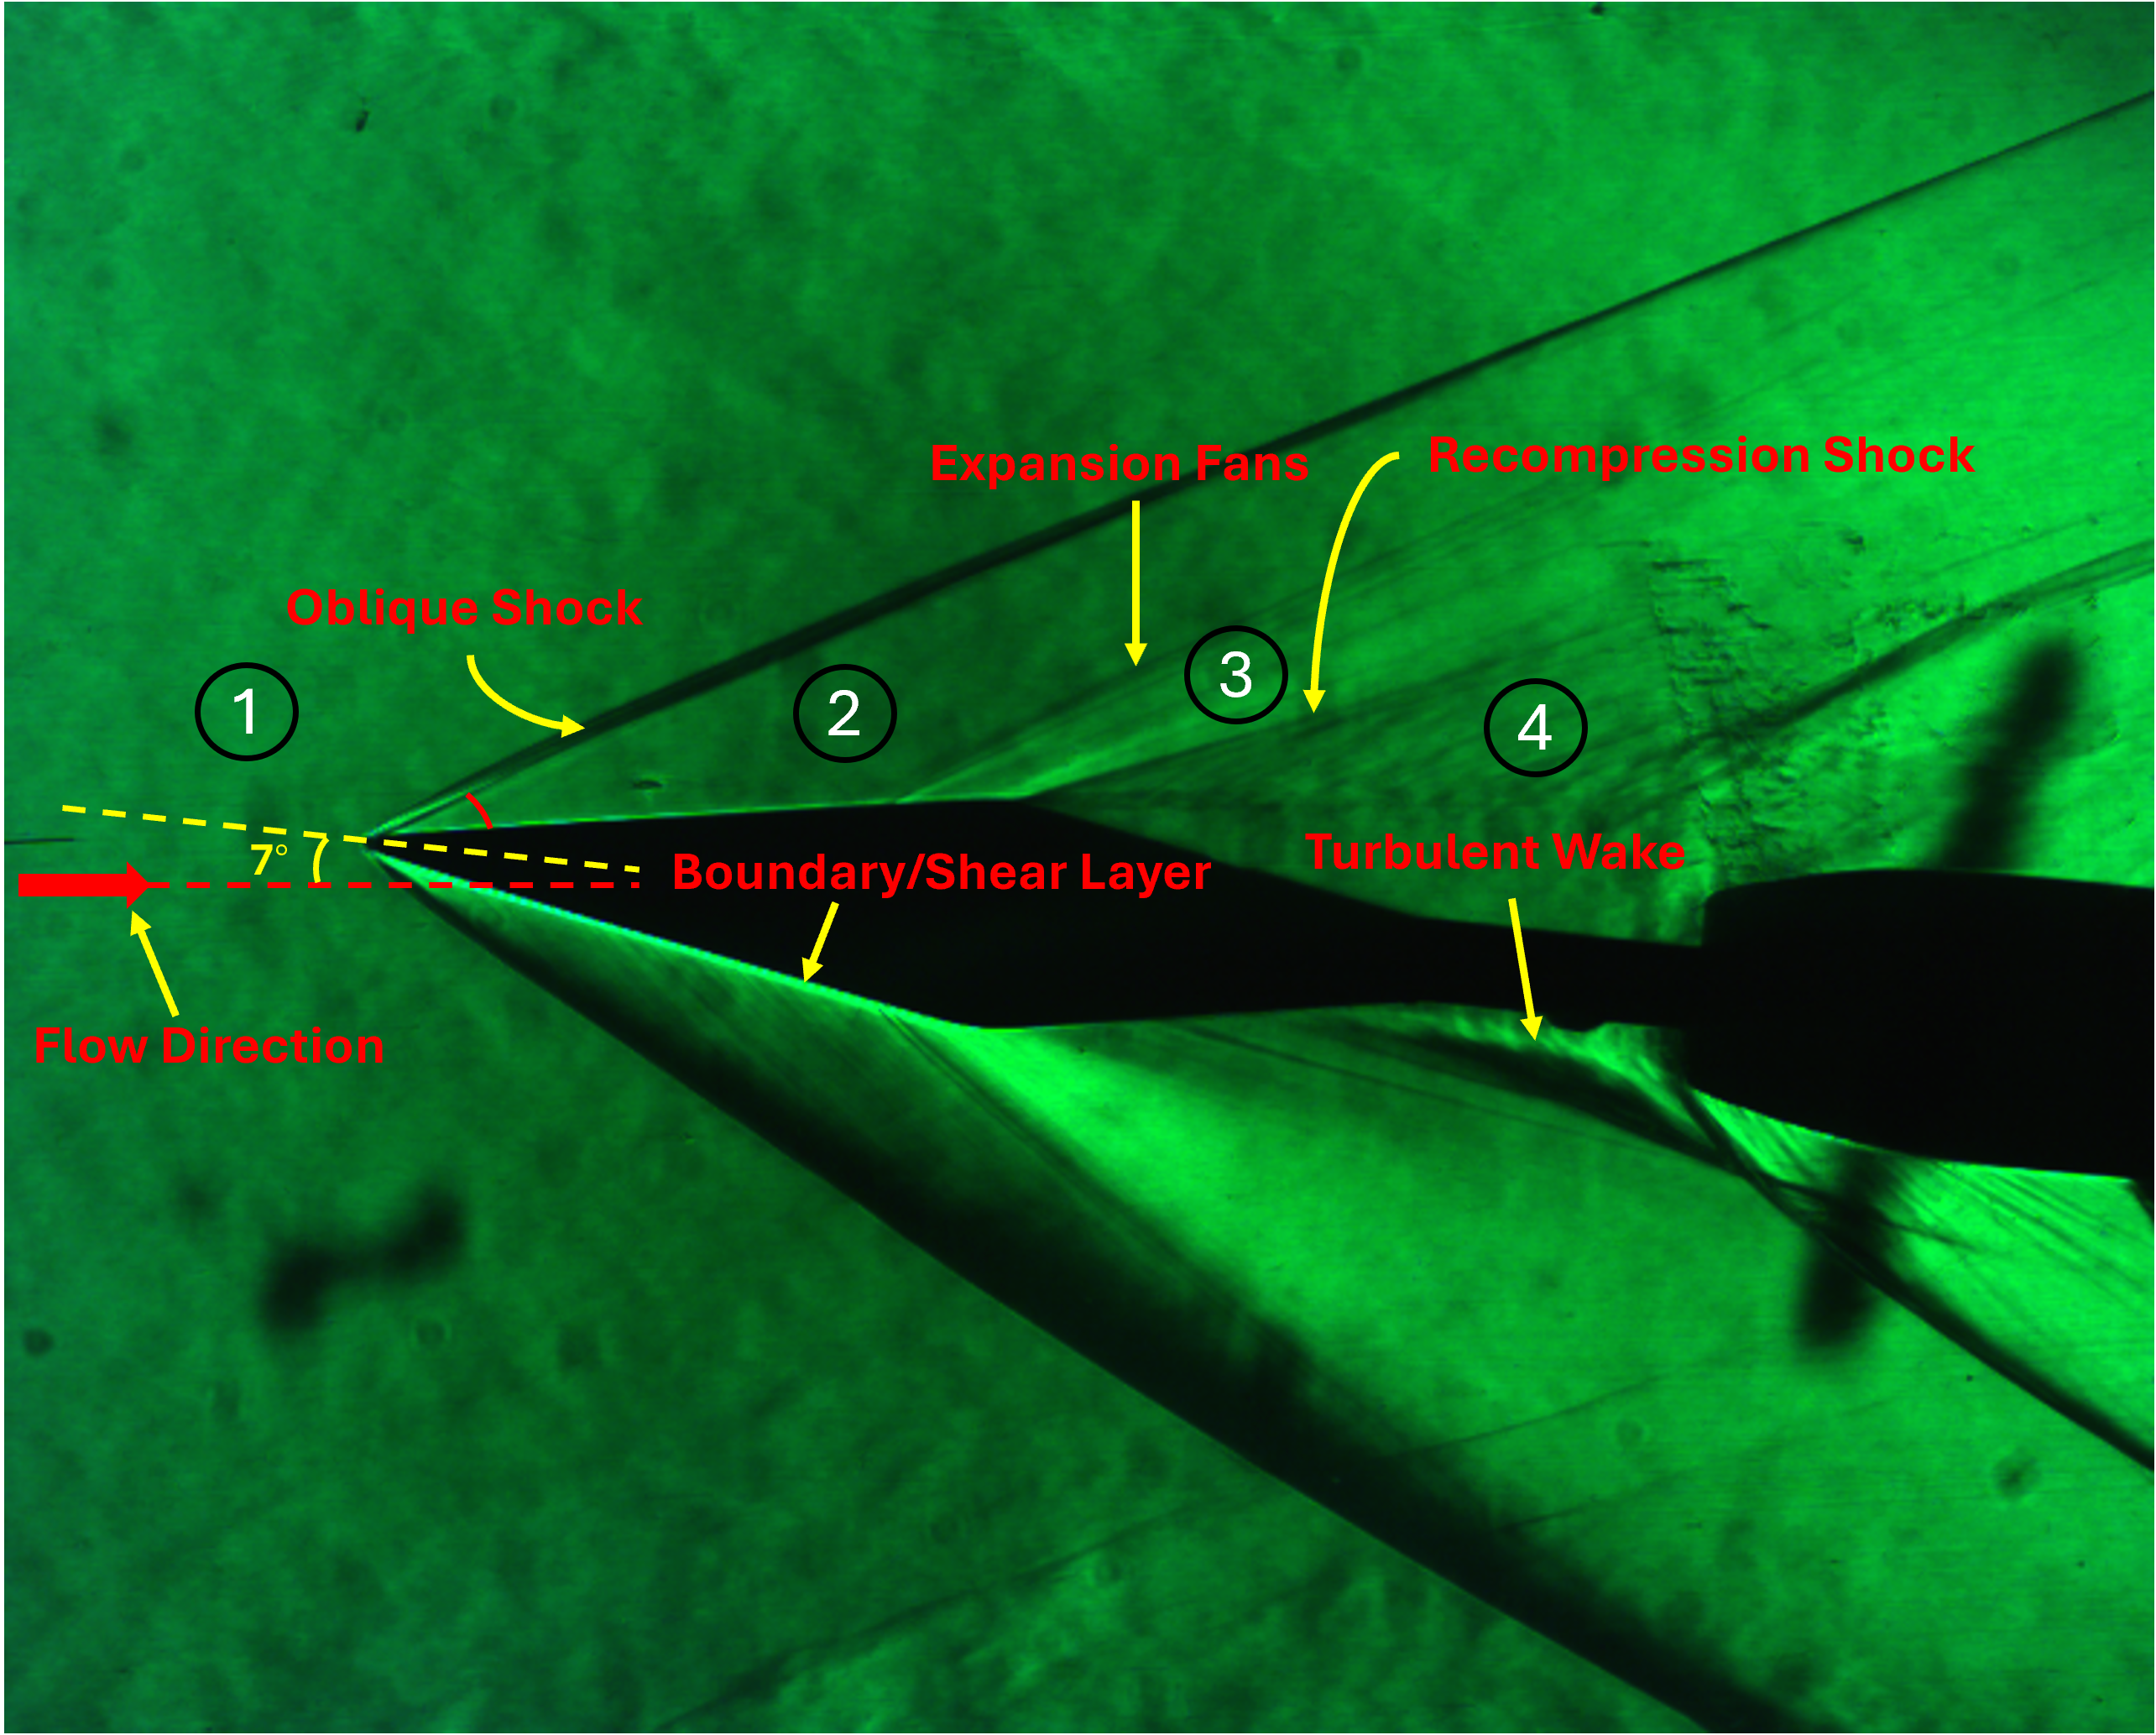
\includegraphics[width=\linewidth]{LabeledImages/Mach3_AoA7.png}
        \caption{Mach 3 flow at $7\degree$ angle of attack}
    \end{subfigure}
    \caption{Diamond Airfoil at different Machs and Angles of Attack}
    \label{images}
\end{figure}

Similarities and Differences between the different flows in Figure \ref{images} : 
\begin{itemize}
    \item Similarities:
    \begin{itemize}
        \item Each flow was visualized using a Vertical Schliern setup.
        \item The density gradients past the shocks and expansions is visibly clear. That is the density increase across the shock and density drop across the P-M fans are shown clearly by the light captured from the image.
        \item In each image there is a visible turbulent wake at the end of the diamond airfoil (zone 4).
        \item In each image, the expansion fans and recompression shocks seem to be occuring earlier than on a theoretical diamond airfoil. This discrepancy may be due to the test article not having sharp edges.
        \item Unlabeled : At the bottom of images (a) and (b) in Figure \ref{images}, a wave reflection can be seen as the shock interacts with the wall enclosing the test section.
    \end{itemize}
    \vspace{10mm}

    \item Differences:
    \begin{itemize}
        \item Between the Mach 2 and Mach 2.5 flows at $0\degree$ angle of attack, you can clearly see the shock angle becoming smaller. In addition, the expansion zone is smaller too.
        \item At Mach 3 and $7\degree$ angle of attack the boundary layer and expansion zone are much tighter on the top of the diamond (top in reference to image; originally the diamond airfoil was tilted $7\degree$ counterclockwise).
        \item The density gradient is much clearer and bigger on the bottom of the diamond airfoil at $7\degree$ angle of attack in Mach 3 flow. More of the flow is hitting that area.
    \end{itemize}
\end{itemize}

As Mach number increases, the shock wave angle decreases (refer to $\theta$-$\beta$-$M$ Relation). These images satisfy shock-expansion theory in this regard. However, as noted previously, the P-M expansion fans and recompression shocks occur much more upstream than shown on a theoretical diamond airfoil.

\subsubsection{Image Correction}
\begin{figure}[H]
    \centering
    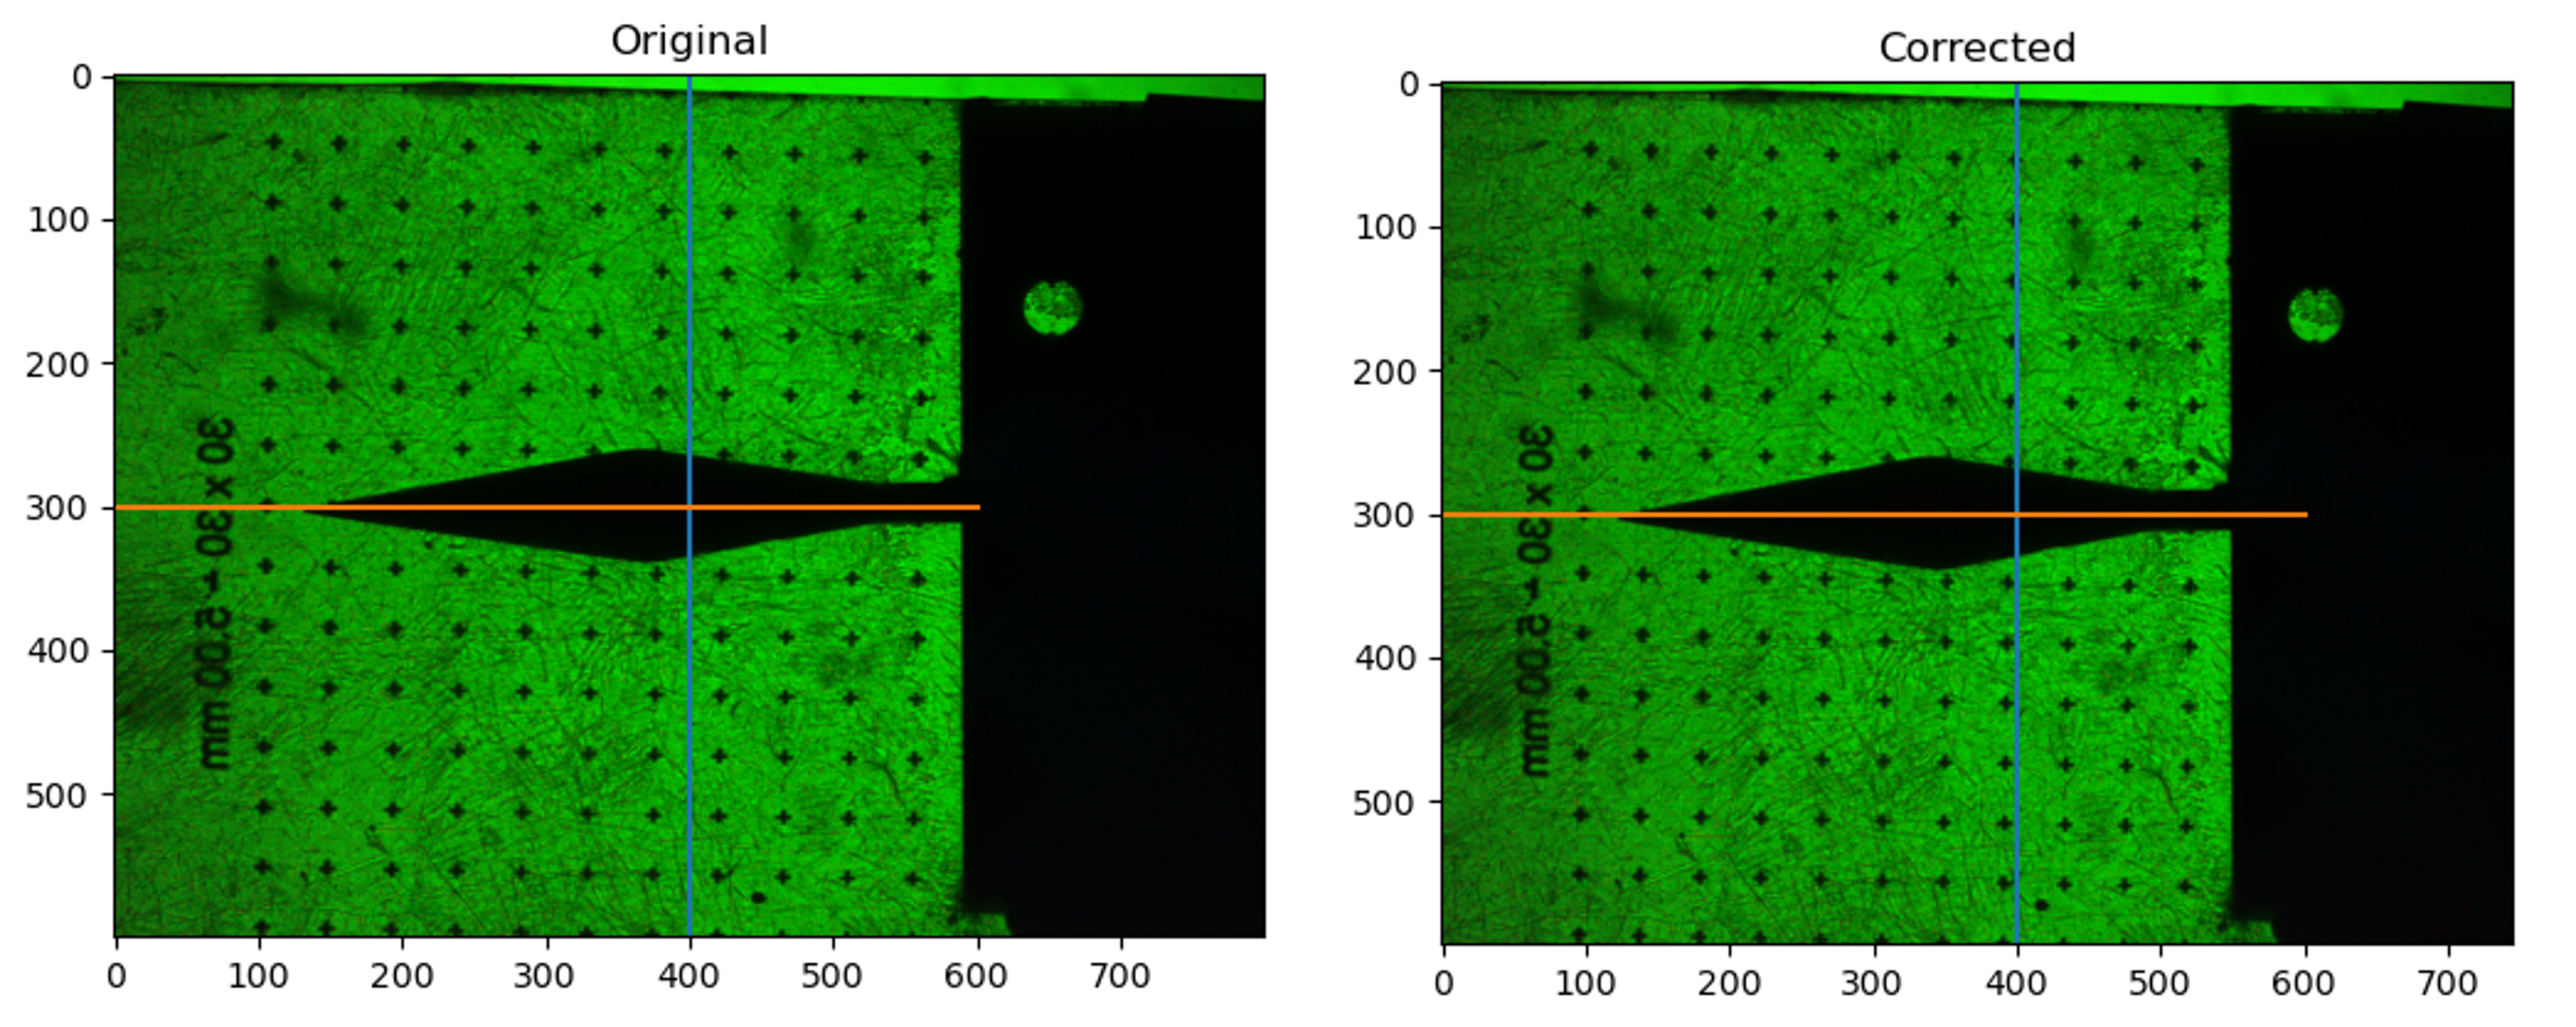
\includegraphics[width = \linewidth]{CorrectedImages/Diamond_GridImage_corrected_vs_raw.png}
    \caption{Corrected wind-off grid image, Raw vs Corrected}
    \label{correction}
\end{figure}

The distortion is not very noticable, however we had to correct for a stretch in the horizontal direction as seen in the images of Figure \ref{correction} and \ref{correctionexample}.
\vspace{5mm}

The raw resolution used was $800$ x $600$ pixels. After correction this became $745$ x $600$ pixels.
\vspace{2.5mm}

A calibration factor was calculated using this formula:
\begin{equation*}
    f = \dfrac{d_{\text{px}}}{n\cdot (5)}
\end{equation*}

The distance between each grid point is $5\, \text{mm}$ and $10$ grid points were used to measure the pixel distance along the grid making $n = 10$. It was found that $f_{x} = 9.06\, \text{pixel/mm}$ and $f_{y} = 8.44\, \text{pixel/mm}$. Thus there were more pixels in the horizontal direction for the same distance on the grid than in the vertical direction. Therefore the horizontal resolution was corrected by $800\cdot (f_{y}/f_{x}) \approx 745\, \text{px}$. Now the grid distance ratio in pixels to millimeter will match for both the horizontal and vertical directions.

\begin{figure}[H]
    \centering
    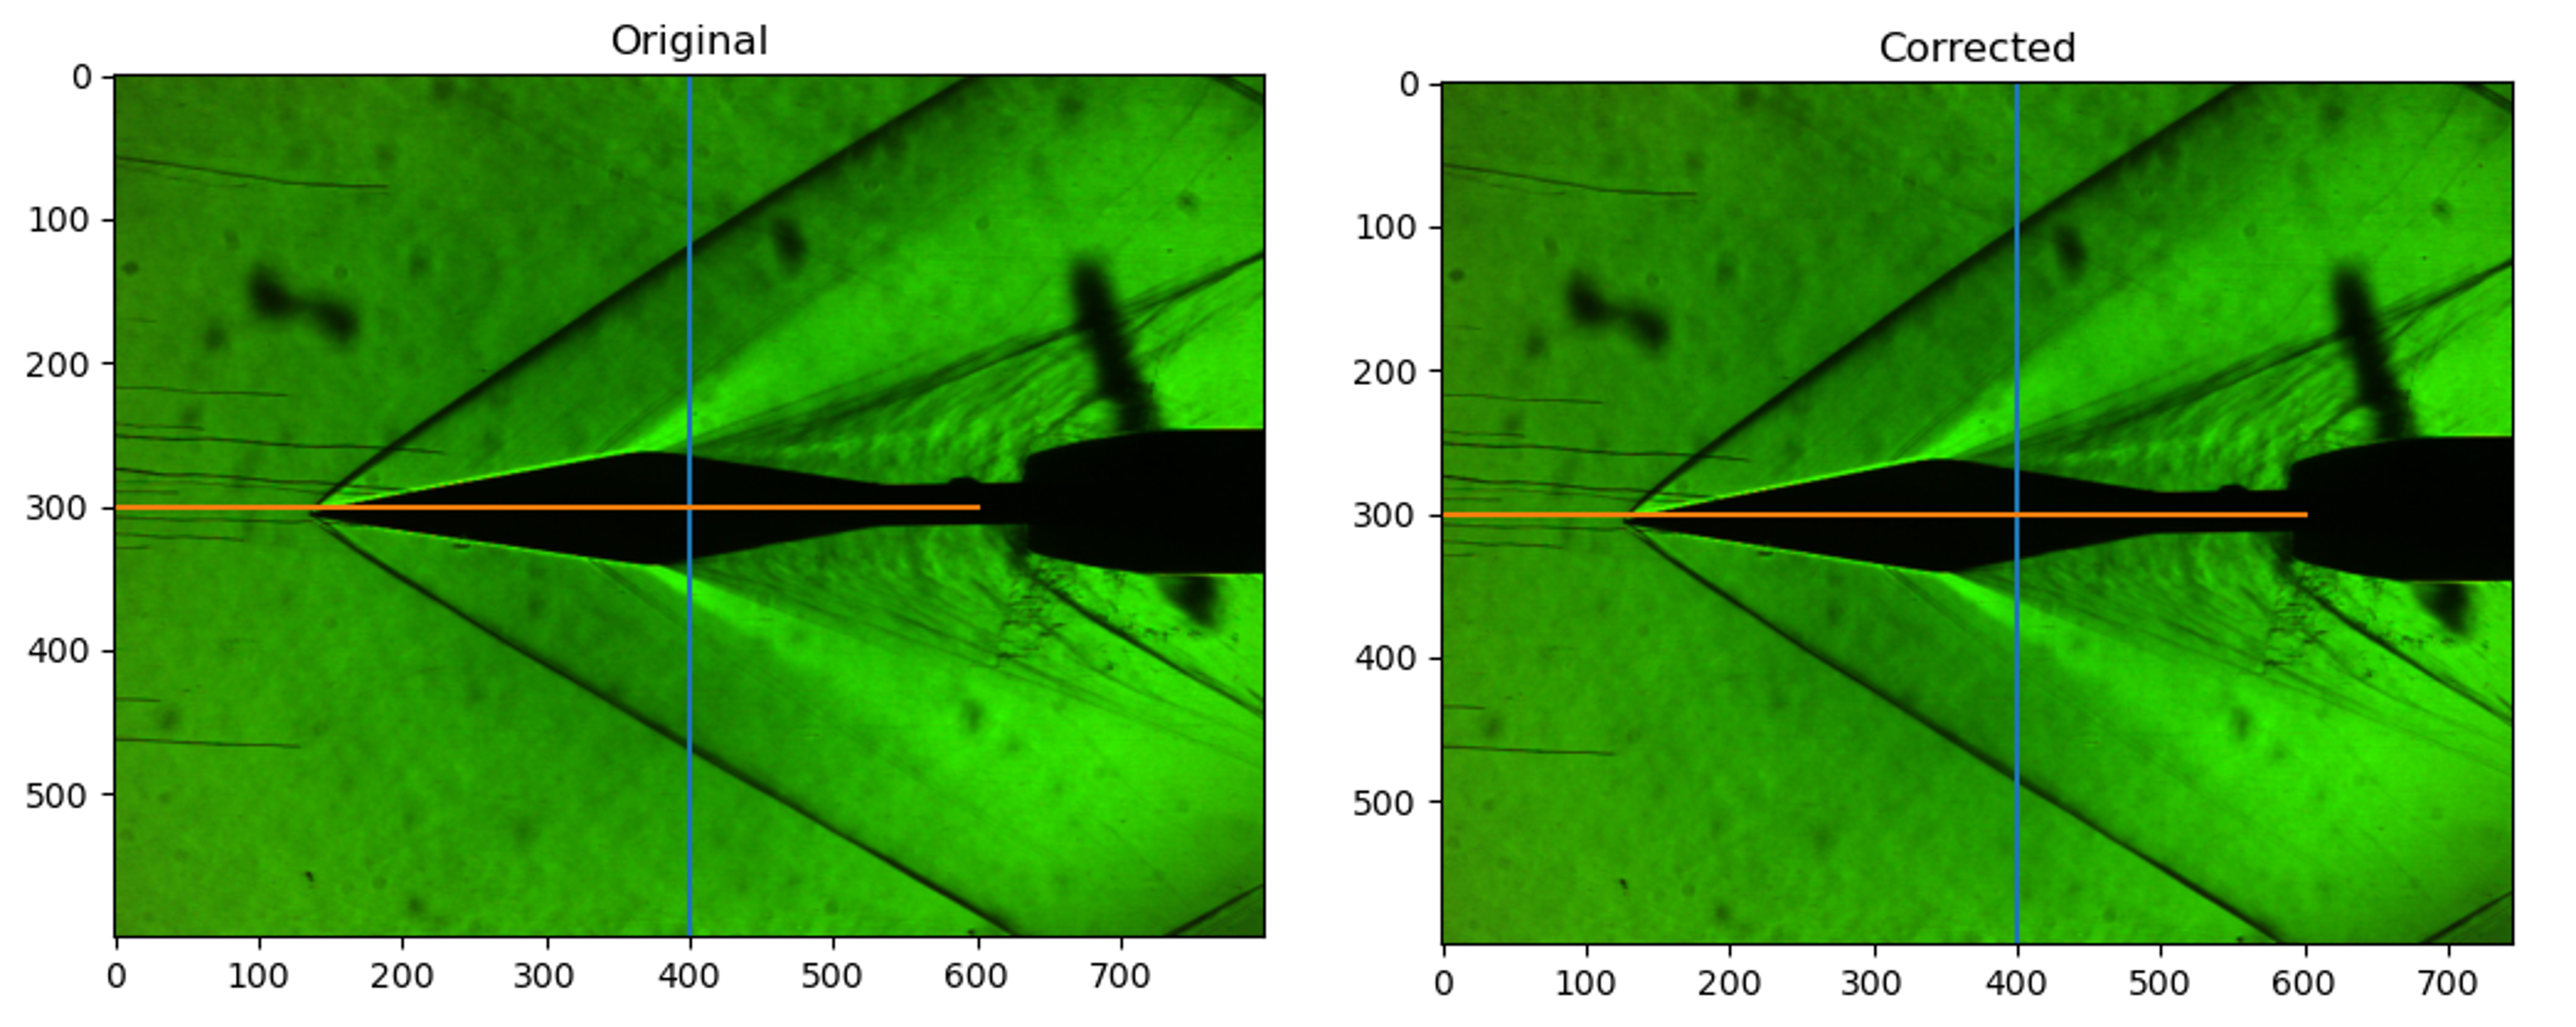
\includegraphics[width = \linewidth]{CorrectedImages/Diamond_AoA0_Mach25_corrected_vs_original.png}
    \caption{Corrected Example with Mach 2.5 flow at $0\degree$ angle of attack, Raw vs Corrected}
    \label{correctionexample}
\end{figure}

\pagebreak

\subsection{True Mach \& Experimental vs Theoeritcal Surface Pressures}

\pagebreak

\subsection{Data Plots}

\subsection{Theoretical Plots}

\pagebreak

\subsection{Center of Pressure}

\pagebreak

\section{Conclusion}

\pagebreak

\section{References}

\pagebreak
\appendix
\pagenumbering{gobble} 
\begin{center}
\vspace*{\fill}
   \Huge \bf Appendix 
\vspace*{\fill}
\end{center}
\pagebreak 


\hypertarget{derivations}{}
\section{Derivations}

Equations for lift and drag analysis:

\begin{equation*}
    C_{l} = \dfrac{l}{\frac{1}{2}\rho_{\infty}U_{\infty}^{2}c} = \dfrac{l}{\frac{1}{2}\gamma P_{\infty} M_{\infty}^{2} c}
\end{equation*}
\vspace{5mm}

\begin{equation*}
    C_{d} = \dfrac{d}{\frac{1}{2}\rho_{\infty}U_{\infty}^{2}c} = \dfrac{d}{\frac{1}{2}\gamma P_{\infty} M_{\infty}^{2} c}
\end{equation*}
\vspace{5mm}

\begin{equation*}
    l = P_{3}z\cos{(\theta + \alpha)} + P_{4}z\cos{(\theta-\alpha)}-P_{1}z\cos{(\theta-\alpha)} - - P_{2}z\sin{(\theta + \alpha)}
\end{equation*}
\vspace{5mm}

\begin{equation*}
    d = P_{1}z\sin{(\theta - \alpha)} + P_{3}z\sin{(\theta + \alpha)} - P_{2}z\sin{(\theta + \alpha)} - P_{4}z\sin{(\theta - \alpha)}
\end{equation*}
\vspace{5mm}

\begin{equation*}
    C_{l} = \dfrac{z}{\frac{1}{2}\gamma P_{\infty} M_{\infty}^{2} c} \left[(P_{3} - P_{2})\cos{(\theta + \alpha)} + (P_{4}-P_{1})\cos{(\theta-\alpha)}\right]
\end{equation*}
\vspace{5mm}

\begin{equation*}
    C_{d} = \dfrac{z}{\frac{1}{2}\gamma P_{\infty} M_{\infty}^{2} c} \left[(P_{3} - P_{2})\sin{(\theta + \alpha)} + (P_{1} - P_{4})\sin{(\theta - \alpha)}\right]
\end{equation*}
\vspace{5mm}

\begin{equation*}
    z = \dfrac{(c/2)}{\cos{(\theta)}}
\end{equation*}
\vspace{5mm}

\begin{equation*}
    C_{l} = \dfrac{1}{\gamma P_{\infty} M_{\infty}^{2} \cos{(\theta)}} \left[(P_{3} - P_{2})\cos{(\theta + \alpha)} + (P_{4}-P_{1})\cos{(\theta-\alpha)}\right]
\end{equation*}
\vspace{5mm}

\begin{equation*}
    C_{d} = \dfrac{1}{\gamma P_{\infty} M_{\infty}^{2} \cos{(\theta)}} \left[(P_{1} - P_{4})\sin{(\theta - \alpha)} + (P_{3} - P_{2})\sin{(\theta + \alpha)}\right]
\end{equation*}
\vspace{5mm}

\end{document}